\documentclass[chaptersright]{informeutn}
\usepackage[utf8]{inputenc}
\usepackage{array}
\usepackage{geometry}
\usepackage[table]{xcolor}
\usepackage{colortbl}
\usepackage{caption}
\usepackage{graphicx}
\usepackage{amsmath}
\usepackage{multirow}
\usepackage{float}

\materia{Dispositivos Electronicos I}
\titulo{Trabajo Practico N°5: TIRISTORES}
\comision{3R2}
\autores{Documentador y operador: Gaston Grasso 401892\\ Coordinador: Angelo Prieto 401012}
\fecha{14-10-2025}


\begin{document}
\maketitle
\tableofcontents

\chapter{Introduccion}

\chapter{SCR}
\section{Condición de disparo y corriente de mantenimiento}
\subsection{Actividad de laboratorio}

\begin{table}[ht!]
    \centering
    \small
    \begin{tabular}{|c|c|c|c|}
       \hline
       $I_G$ [mA] & $V_{CC}$ [V] & $I_{AK}$ [mA] & $V_{AK}$ [V] \\
       \hline
        2.92 & 600 & 127.51 & 0.7 \\
        2.96 & 465 & 98.79 & 0.7 \\
        2.98 & 398 & 84.53 & 0.7 \\
        3.00 & 345 & 73.25 & 0.7 \\
        3.02 & 295 & 62.62 & 0.7 \\
       \hline
    \end{tabular}
    \caption{relevamiento de disparo del SCR para diferentes valores de $I_G$.}
\end{table}

\subsection{Actividad de simulación}

\section{Obtención de curva característica}
\subsection{Actividad de laboratorio}

\begin{figure}[h]
    \centering
     \begin{tikzpicture}
        % Paths, nodes and wires:
        \draw (-6.38, 2) to[american resistor, l={$R_1$}] (-6.38, 4);
        \draw (-6.38, 1) to[american potentiometer] (-6.38, -1);
        \draw (-3.38, -0) to[american resistor, l={$R_G$}] (-5.38, -0);
        \draw (-2.88, -0) to[ammeter, l={$I_G$}] (-0.88, -0);
        \draw (-0.88, -0) to[normal open switch] (1.37, -0);
        \draw (2.154, 2.295) to[empty thyristor, mirror] (2.134, -0.905);
        \draw (2.154, 2.295) to[american resistor, l={$R_2$}] (2.154, 4.295);
        \draw (2.12, -3) to[ammeter, l={$I_{AK}$}] (2.134, -0.905);
        \draw (4.12, -1) to[voltmeter, l={$V_{AK}$}] (4.12, 1);
        \draw (6.12, -1) to[voltmeter, l={$V_{CC}$}] (6.12, 1);
        \draw (4.12, 1) |- (2.12, 2);
        \draw (6.12, 1) |- (2.154, 4.295);
        \draw (4.12, -1) -| (4.12, -3);
        \draw (6.12, -1) -| (6.12, -3);
        \draw (6.12, -3) |- (-6.38, -3);
        \draw (-6.38, -3) -| (-6.38, -1);
        \draw (-6.38, 1) -| (-6.38, 2);
        \draw (2.154, 4.295) |- (2.12, 5);
        \draw (-6.38, 4) -| (-6.38, 5);
        \draw (-5.82, -0) -- (-5.38, -0);
        \draw (-3.13, -3) to[voltmeter, l={$V_G$}] (-3.13, -0);
        \draw (-3.38, -0) -- (-2.88, -0);
        \node[vcc](N1) at (-6.38, 5){} node[anchor=south] at (N1.text){$20V$};
        \node[vcc](N2) at (2.154, 5){} node[anchor=south] at (N2.text){$V_{CC}$};
        \node[ground] at (2.12, -3){};
    \end{tikzpicture}
    \caption{circuito implementado en el laboratorio.}
\end{figure}

\begin{table}[h]
    \centering
    \small
    \begin{tabular}{|cc|cc|cc|cc|cc|}
        \hline
        \multicolumn{2}{|c|}{$I_{G} = 2.92mA\,$}
        & \multicolumn{2}{c|}{$I_{G} = 2.96mA\,$}
        & \multicolumn{2}{c|}{$I_{G} = 2.98mA\,$}
        & \multicolumn{2}{c|}{$I_{G} = 3.00mA\,$}
        & \multicolumn{2}{c|}{$I_{G} = 3.02mA\,$}\\
        \hline
        $V_{AK}$ [V] & $I_{AK}$ [mA] & $V_{AK}$ [V] & $I_{AK}$ [mA] & $V_{AK}$ [V] & $I_{AK}$ [mA] & $V_{AK}$ [V] & $I_{AK}$ [mA] & $V_{AK}$ [V] & $I_{AK}$ [mA] \\
        \hline
        0    & 0.000  & 0      & 0.000  & 0     & 0.000 & 0     & 0.000& 0    & 0.000 \\
        50   & 0.000  & 50     & 0.000  & 50    & 0.000 & 50    & 0.000& 50   & 0.000 \\
        100  & 0.000  & 98     & 0.000  & 100   & 0.000 & 100   & 0.000& 98.3 & 0.000 \\
        200  & 0.000  & 148    & 0.000  & 147.5 & 0.000 & 148.2 & 0.000& 148  & 0.000 \\
        300  & 0.000  & 197.5  & 0.000  & 198   & 0.000 & 200   & 0.000& 200  & 0.000 \\
        350  & 0.000  & 247.5  & 0.000  & 250   & 0.000 & 247   & 0.000& 247.5& 0.638\\
        400  & 0.000  & 296.1  & 0.000  & 296.3 & 0.000 & 297   & 0.000& 297.5& 0.53 \\
        450  & 0.000  & 343.5  & 0.000  & 346   & 0.000 & 320.8 & 0.89 & 0.7  & 62.62 \\
        500  & 0.000  & 392.4  & 0.000  & 0.7   & 84.53 & 0.7   & 73.25  & -  &- \\
        550  & 0.000  & 443.6  & 0.000  & -     & -     & -   & - & - & - \\
        600  & 0.000  & 0.7    & 98.79  & -     & -     & -   & - & - & - \\
        0.7 & 127.51 &-&-&-&-&-&-&-&-\\
        \hline
    \end{tabular}
    \caption{Tabla de $I_{AK} = f(V_{AK})$ para distintos valores de $I_{G}$.}
\end{table}

\begin{figure}[h]
    \centering
    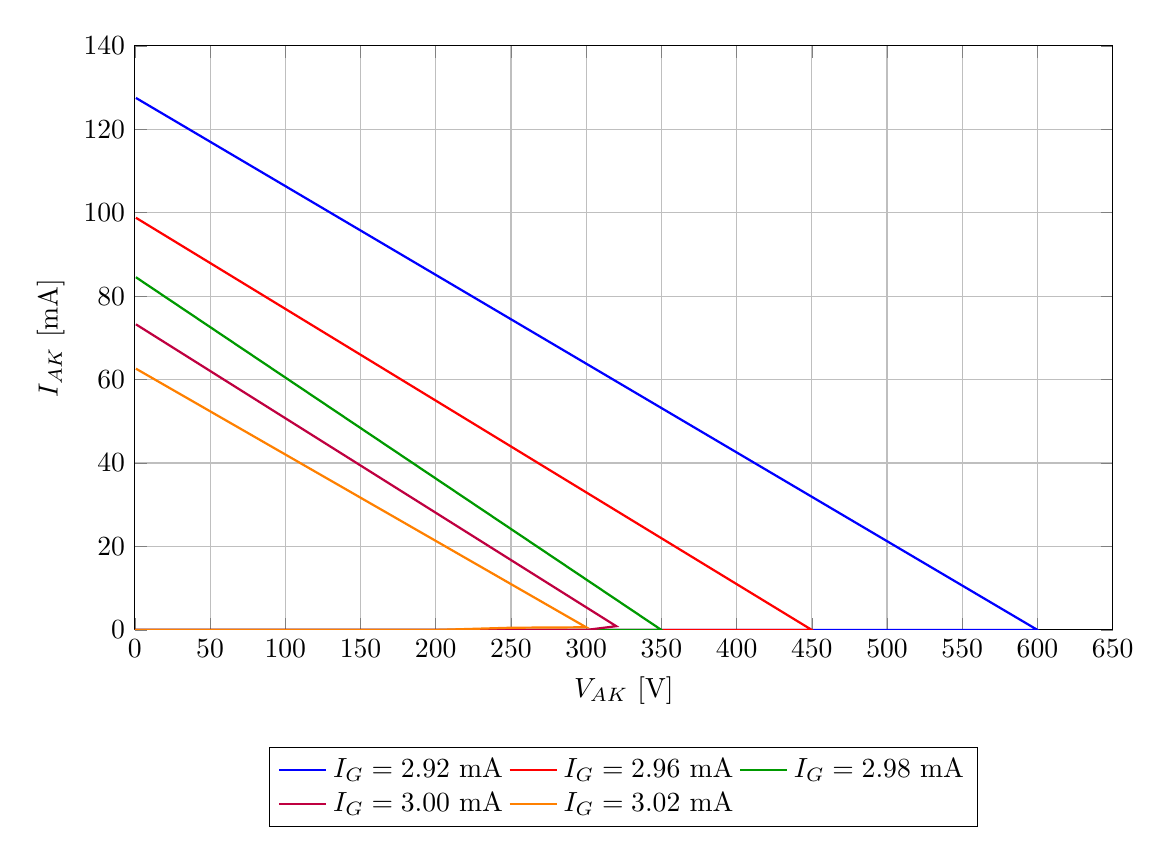
\begin{tikzpicture}
    \begin{axis}[
        width=14cm,
        height=9cm,
        xlabel={$V_{AK}$ [V]},
        ylabel={$I_{AK}$ [mA]},
        grid=both,
        ymin=0, ymax=140,
        xmin=0, xmax=650,
        legend style={at={(0.5,-0.2)},anchor=north,legend columns=3},
    ]

    % ---- IG = 2.92 mA ----
    \addplot[blue, thick] coordinates {
        (0,0) (50,0) (100,0) (200,0) (300,0) (400,0) (500,0) (600,0)
        (0.7,127.51)
    };
    \addlegendentry{$I_G = 2.92$ mA}

    % ---- IG = 2.96 mA ----
    \addplot[red, thick] coordinates {
        (0,0) (50,0) (100,0) (150,0) (200,0) (250,0) (300,0)
        (350,0) (400,0) (450,0) (0.7, 98.79)
    };
    \addlegendentry{$I_G = 2.96$ mA}

    % ---- IG = 2.98 mA ----
    \addplot[green!60!black, thick] coordinates {
        (0,0) (50,0) (100,0) (150,0) (200,0) (250,0) (300,0) (350,0) (0.7,84.53)
    };
    \addlegendentry{$I_G = 2.98$ mA}

    % ---- IG = 3.00 mA ----
    \addplot[purple, thick] coordinates {
        (0,0) (50,0) (100,0) (150,0) (200,0) (250,0) (300,0) (320,0.9)
        (0.7,73.25)
    };
    \addlegendentry{$I_G = 3.00$ mA}

    % ---- IG = 3.02 mA ----
    \addplot[orange, thick] coordinates {
        (0,0) (50,0) (100,0) (150,0) (200,0) (250,0.53) (300,0.638)
        (0.7,62.62)
    };
    \addlegendentry{$I_G = 3.02$ mA}

    \end{axis}
\end{tikzpicture}
\caption{Curvas características $I_{AK}(V_{AK})$ del SCR para distintos $I_G$.}
\end{figure}



\section{Funcionamiento con corriente alterna}
\subsection{Actividad de simulación}

\chapter{DIAC}
Objetivo: determinar la polarización y funcionamiento del DIAC.
\section{Actividad de laboratorio}
\begin{figure}[ht!]
    \centering
    \begin{tikzpicture}
        % Paths, nodes and wires:
        \draw (-1.75, -1) to[full bidirectionaldiode] (-1.75, 1);
        \draw (1.25, -1) to[voltmeter, l={$V_2$}] (1.25, 1);
        \draw (-1.75, 1) to[american resistor, l={$R$}] (-1.75, 3);
        \node[vcc](N1) at (-1.75, 3.5){} node[anchor=south] at (N1.text){$V_{CC}$};
        \draw (-1.75, 1) -- (1.25, 1);
        \draw (-1.75, -1) -- (1.25, -1);
        \draw (3.25, -0) to[voltmeter, l={$V_1$}] (3.25, 2);
        \draw (-1.75, 3) -| (3.25, 2);
        \draw (-1.75, -3) to[ammeter] (-1.75, -1);
        \node[ground] at (-1.75, -3){};
        \draw (-1.75, 3) -| (-1.75, 3.5);
        \draw (3.25, -0) |- (-1.75, -1.25);
    \end{tikzpicture}
    \caption{circuito implementado en el laboratorio.}
\end{figure}

\begin{table}[ht!]
    \centering
    \small
    \begin{tabular}{|c|c|c|c|c|c|c|c|c|c|}
       \hline
       $V_{CC}$ [V] & 0 & 10 & 20 & 30 & 32 & 34 & 40 & 45 & 50 \\
       \hline
       $V_{AK}$ [V] & 0 & 10 & 20 & 30 & 23.8 & 23.4 & 22.6 & 22.2 & 21.9 \\
       \hline
       $I_{AK}$ [mA] & 0 & 0 & 0 & 0 & 1.74 & 2.24 & 3.72 & 4.9 & 5.92 \\
       \hline
    \end{tabular}
    \caption{relevamiento de disparo del SCR para diferentes valores de $I_G$.}
\end{table}

\begin{figure}[ht!]
  \centering
  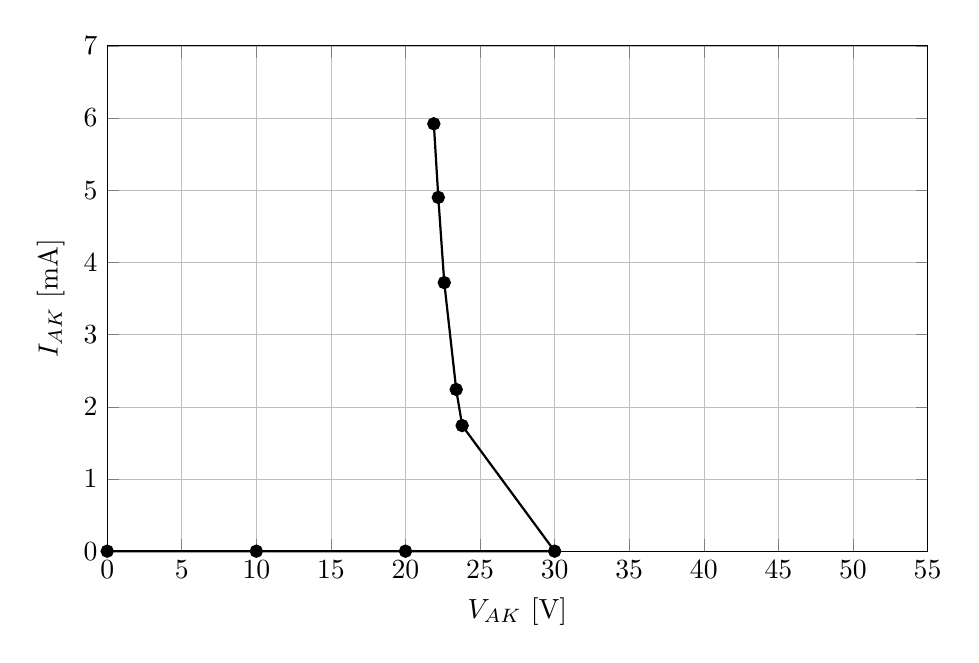
\begin{tikzpicture}
    \begin{axis}[
      width=12cm, height=8cm,
      xlabel={$V_{AK}$ [V]},
      ylabel={$I_{AK}$ [mA]},
      xmin=0, xmax=55,
      ymin=0, ymax=7,
      grid=both,
      grid style={line width=.1pt, draw=gray!30},
      major grid style={line width=.2pt,draw=gray!50},
      legend pos= north west,
      enlargelimits=false,
      clip=false,
    ]

    % Datos (ordenados para la gráfica)
    \addplot[
      mark=*,
      mark options={fill=white},
      thick,
    ] coordinates {
      (0,0)
      (10,0)
      (20,0)
      (30,0)
      (23.8,1.74)
      (23.4,2.24)
      (22.6,3.72)
      (22.2,4.90)
      (21.9,5.92)
      };

    % Marcar los puntos originales (más visibles)
    \addplot[only marks, mark=*, mark size=2pt] coordinates {
      (0,0) (10,0) (20,0) (21.9,5.92) (22.2,4.90) (22.6,3.72)
      (23.4,2.24) (23.8,1.74) (30,0) 
    };

    \end{axis}
  \end{tikzpicture}
  \caption{Curva $I_{AK}$ vs $V_{AK}$ del DIAC (datos experimentales).}
  \label{fig:diac-IV}
\end{figure}

\chapter{TRIAC}
\section{Polarización y funcionamiento}
\subsection{Actividad de laboratorio}
\begin{figure}[ht]
    \centering
    \begin{tikzpicture}
        % Paths, nodes and wires:
        \draw (0.02, 2) to[american resistor, l={$R$}] (0.02, 4);
        \node[ground] at (0.02, -3.7){};
        \draw (-1.253, -0.018) to[full bidirectionaldiode] (-3.253, -0.018);
        \draw (0, -1.75) to[full triac] (0.02, 0.3);
        \draw (-5, -0) to[ammeter, l={$I_G$}] (-3.5, -0);
        \draw (-6, -1) to[american potentiometer, mirror] (-6, 1);
        \draw (0.02, 0.3) |- (0, 2);
        \draw (-6, 1) -- (-6, 2) -- (0, 2);
        \draw (0.02, -3.7) to[ammeter, l={$I_A$}] (0, -1.75);
        \draw (2.25, -2) to[voltmeter, l={$V_{CC}$}] (2.25, 1);
        \draw (2.25, -2) |- (0.02, -3.7);
        \draw (2.25, 1) |- (0.02, 4);
        \draw (-6, -1) |- (0.02, -3.7);
        \node[vcc] at (0, 4){};
        \node[vcc](N1) at (0.02, 4){} node[anchor=south] at (N1.text){$V_{CC}$};
        \draw (-5, -0) -- (-5.44, -0);
        \draw (-3.25, -0) -- (-3.5, -0);
        \draw (-1.253, -0.018) -- (-0.753, -0.018);
    \end{tikzpicture}
    \caption{circuito implementado en el laboratorio.}
\end{figure}

\section{Aplicación: control de disparo (Dimmer)}
\subsection{Actividad de laboratorio}

\chapter{Interpretación de las especificaciones del fabricante}

\chapter{Conclusión}
\end{document}
